% Options for packages loaded elsewhere
\PassOptionsToPackage{unicode}{hyperref}
\PassOptionsToPackage{hyphens}{url}
%
\documentclass[
  letterpaper,
]{scrbook}

\usepackage{amsmath,amssymb}
\usepackage{lmodern}
\usepackage{iftex}
\ifPDFTeX
  \usepackage[T1]{fontenc}
  \usepackage[utf8]{inputenc}
  \usepackage{textcomp} % provide euro and other symbols
\else % if luatex or xetex
  \usepackage{unicode-math}
  \defaultfontfeatures{Scale=MatchLowercase}
  \defaultfontfeatures[\rmfamily]{Ligatures=TeX,Scale=1}
\fi
% Use upquote if available, for straight quotes in verbatim environments
\IfFileExists{upquote.sty}{\usepackage{upquote}}{}
\IfFileExists{microtype.sty}{% use microtype if available
  \usepackage[]{microtype}
  \UseMicrotypeSet[protrusion]{basicmath} % disable protrusion for tt fonts
}{}
\makeatletter
\@ifundefined{KOMAClassName}{% if non-KOMA class
  \IfFileExists{parskip.sty}{%
    \usepackage{parskip}
  }{% else
    \setlength{\parindent}{0pt}
    \setlength{\parskip}{6pt plus 2pt minus 1pt}}
}{% if KOMA class
  \KOMAoptions{parskip=half}}
\makeatother
\usepackage{xcolor}
\setlength{\emergencystretch}{3em} % prevent overfull lines
\setcounter{secnumdepth}{5}
% Make \paragraph and \subparagraph free-standing
\ifx\paragraph\undefined\else
  \let\oldparagraph\paragraph
  \renewcommand{\paragraph}[1]{\oldparagraph{#1}\mbox{}}
\fi
\ifx\subparagraph\undefined\else
  \let\oldsubparagraph\subparagraph
  \renewcommand{\subparagraph}[1]{\oldsubparagraph{#1}\mbox{}}
\fi


\providecommand{\tightlist}{%
  \setlength{\itemsep}{0pt}\setlength{\parskip}{0pt}}\usepackage{longtable,booktabs,array}
\usepackage{calc} % for calculating minipage widths
% Correct order of tables after \paragraph or \subparagraph
\usepackage{etoolbox}
\makeatletter
\patchcmd\longtable{\par}{\if@noskipsec\mbox{}\fi\par}{}{}
\makeatother
% Allow footnotes in longtable head/foot
\IfFileExists{footnotehyper.sty}{\usepackage{footnotehyper}}{\usepackage{footnote}}
\makesavenoteenv{longtable}
\usepackage{graphicx}
\makeatletter
\def\maxwidth{\ifdim\Gin@nat@width>\linewidth\linewidth\else\Gin@nat@width\fi}
\def\maxheight{\ifdim\Gin@nat@height>\textheight\textheight\else\Gin@nat@height\fi}
\makeatother
% Scale images if necessary, so that they will not overflow the page
% margins by default, and it is still possible to overwrite the defaults
% using explicit options in \includegraphics[width, height, ...]{}
\setkeys{Gin}{width=\maxwidth,height=\maxheight,keepaspectratio}
% Set default figure placement to htbp
\makeatletter
\def\fps@figure{htbp}
\makeatother
\newlength{\cslhangindent}
\setlength{\cslhangindent}{1.5em}
\newlength{\csllabelwidth}
\setlength{\csllabelwidth}{3em}
\newlength{\cslentryspacingunit} % times entry-spacing
\setlength{\cslentryspacingunit}{\parskip}
\newenvironment{CSLReferences}[2] % #1 hanging-ident, #2 entry spacing
 {% don't indent paragraphs
  \setlength{\parindent}{0pt}
  % turn on hanging indent if param 1 is 1
  \ifodd #1
  \let\oldpar\par
  \def\par{\hangindent=\cslhangindent\oldpar}
  \fi
  % set entry spacing
  \setlength{\parskip}{#2\cslentryspacingunit}
 }%
 {}
\usepackage{calc}
\newcommand{\CSLBlock}[1]{#1\hfill\break}
\newcommand{\CSLLeftMargin}[1]{\parbox[t]{\csllabelwidth}{#1}}
\newcommand{\CSLRightInline}[1]{\parbox[t]{\linewidth - \csllabelwidth}{#1}\break}
\newcommand{\CSLIndent}[1]{\hspace{\cslhangindent}#1}

\usepackage{makeidx}
\makeindex
\makeatletter
\makeatother
\makeatletter
\@ifpackageloaded{bookmark}{}{\usepackage{bookmark}}
\makeatother
\makeatletter
\@ifpackageloaded{caption}{}{\usepackage{caption}}
\AtBeginDocument{%
\ifdefined\contentsname
  \renewcommand*\contentsname{Table of contents}
\else
  \newcommand\contentsname{Table of contents}
\fi
\ifdefined\listfigurename
  \renewcommand*\listfigurename{List of Figures}
\else
  \newcommand\listfigurename{List of Figures}
\fi
\ifdefined\listtablename
  \renewcommand*\listtablename{List of Tables}
\else
  \newcommand\listtablename{List of Tables}
\fi
\ifdefined\figurename
  \renewcommand*\figurename{Figure}
\else
  \newcommand\figurename{Figure}
\fi
\ifdefined\tablename
  \renewcommand*\tablename{Table}
\else
  \newcommand\tablename{Table}
\fi
}
\@ifpackageloaded{float}{}{\usepackage{float}}
\floatstyle{ruled}
\@ifundefined{c@chapter}{\newfloat{codelisting}{h}{lop}}{\newfloat{codelisting}{h}{lop}[chapter]}
\floatname{codelisting}{Listing}
\newcommand*\listoflistings{\listof{codelisting}{List of Listings}}
\makeatother
\makeatletter
\@ifpackageloaded{caption}{}{\usepackage{caption}}
\@ifpackageloaded{subcaption}{}{\usepackage{subcaption}}
\makeatother
\makeatletter
\@ifpackageloaded{tcolorbox}{}{\usepackage[many]{tcolorbox}}
\makeatother
\makeatletter
\@ifundefined{shadecolor}{\definecolor{shadecolor}{rgb}{.97, .97, .97}}
\makeatother
\makeatletter
\makeatother
\ifLuaTeX
  \usepackage{selnolig}  % disable illegal ligatures
\fi
\IfFileExists{bookmark.sty}{\usepackage{bookmark}}{\usepackage{hyperref}}
\IfFileExists{xurl.sty}{\usepackage{xurl}}{} % add URL line breaks if available
\urlstyle{same} % disable monospaced font for URLs
\hypersetup{
  pdftitle={Fehlerlinguistik},
  pdfauthor={Teodor Petrič},
  hidelinks,
  pdfcreator={LaTeX via pandoc}}

\title{Fehlerlinguistik}
\usepackage{etoolbox}
\makeatletter
\providecommand{\subtitle}[1]{% add subtitle to \maketitle
  \apptocmd{\@title}{\par {\large #1 \par}}{}{}
}
\makeatother
\subtitle{Versprecher und andere Fehlerarten im Deutschen (und
Slowenischen)}
\author{Teodor Petrič}
\date{2022-09-26}

\begin{document}
\frontmatter
\maketitle
\ifdefined\Shaded\renewenvironment{Shaded}{\begin{tcolorbox}[frame hidden, interior hidden, breakable, borderline west={3pt}{0pt}{shadecolor}, sharp corners, enhanced, boxrule=0pt]}{\end{tcolorbox}}\fi

\renewcommand*\contentsname{Table of contents}
{
\setcounter{tocdepth}{2}
\tableofcontents
}
\mainmatter
\bookmarksetup{startatroot}

\hypertarget{section}{%
\chapter*{.}\label{section}}
\addcontentsline{toc}{chapter}{.}

\begin{figure}

{\centering 

\href{https://www.clipartmax.com/}{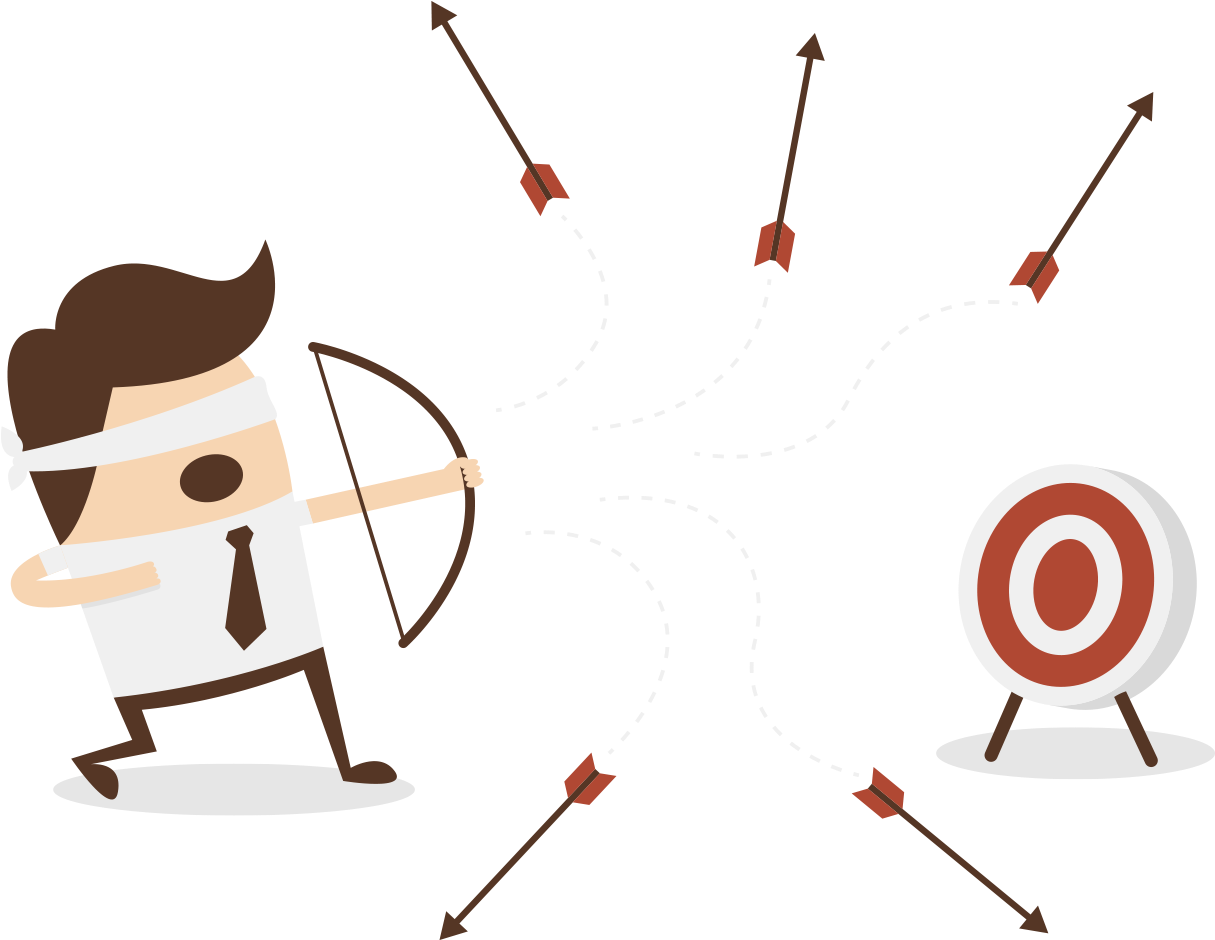
\includegraphics[width=1\textwidth,height=\textheight]{./pictures/clipart2906322_personal_use_only.png}}

}

\end{figure}

\bookmarksetup{startatroot}

\hypertarget{sec-vorwort}{%
\chapter*{Vorwort}\label{sec-vorwort}}
\addcontentsline{toc}{chapter}{Vorwort}

Dieses Buch ist eine Einführung in die Fehlerlinguistik, und zwar unter
besonderer Berücksichtigung von Versprechern im Deutschen und
Slowenischen.

\texttt{Quarto\ Book} \url{https://quarto.org/}

\part{Teil 1:Versprecher}

\hypertarget{sec-einfuhrung}{%
\chapter{Einführung}\label{sec-einfuhrung}}

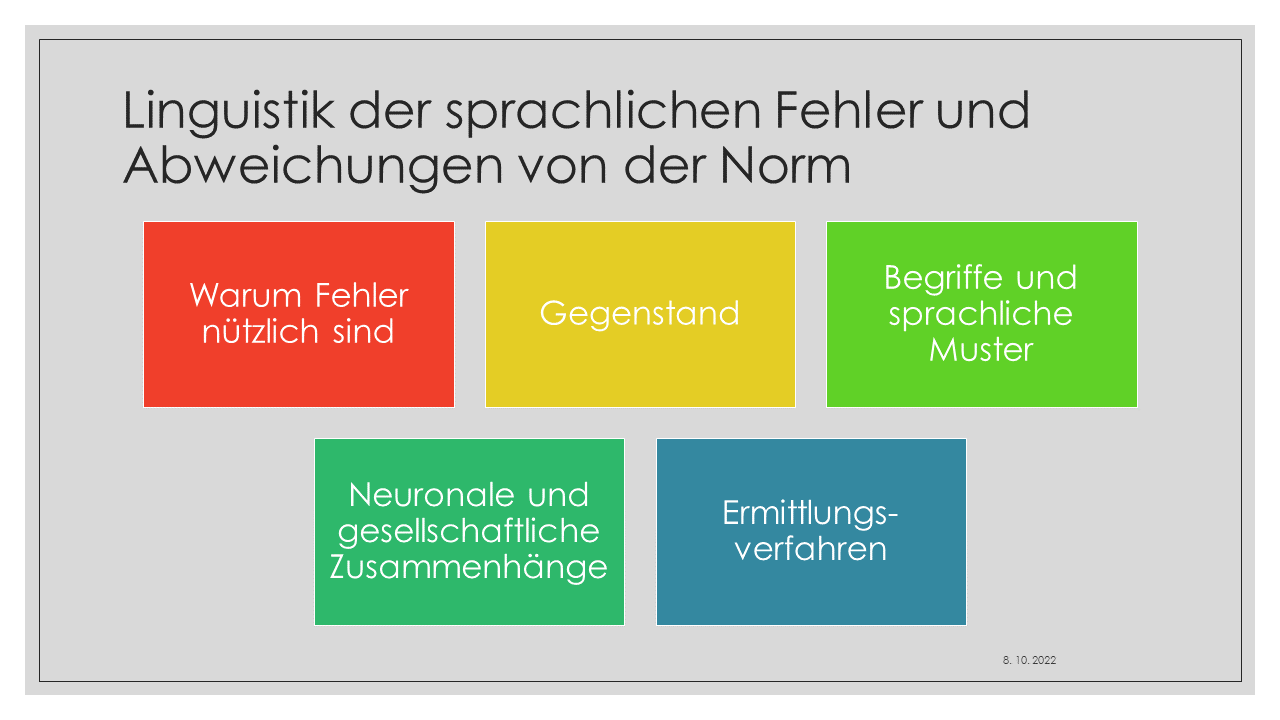
\includegraphics[width=1\textwidth,height=\textheight]{./pictures/Diapozitiv5.PNG}

In diesem Einführungskurs machen wir Sie mit grundlegenden Methoden zur
Erfassung von linguistischen Merkmalen in deutschen (und in einigen
Abschnitten auch mit slowenischen) Texten bekannt..\footnote{Dieses Buch
  wurde mit \texttt{Quarto} \url{https://quarto.org/docs/books/}
  zusammengestellt.}

Hinweise\footnote{Clipart von \url{https://www.clipartmax.com/}}:

Das ist eine Definition (rmdnote).

Das ist ein Tip oder eine Info (rmdtip).

Das ist ein Arbeitsvorschlag (rmdrobot).

Das ist der RStudio Logotyp (rmdrstudio).

Das ist eine Warnung (rmdwarning).

Das ist eine Fehlermeldung (rmderror).

\hypertarget{sec-gegenstand}{%
\chapter{Gegenstand}\label{sec-gegenstand}}

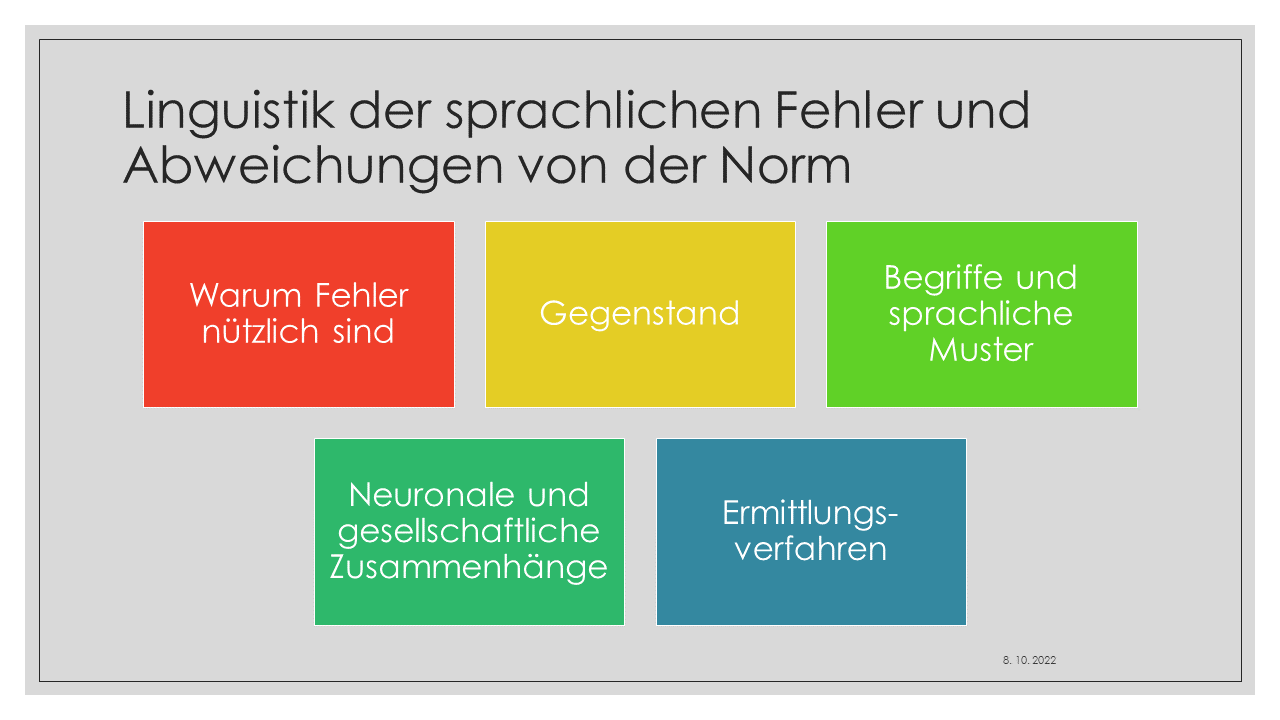
\includegraphics[width=1\textwidth,height=\textheight]{./pictures/Diapozitiv5.PNG}

In diesem Einführungskurs machen wir Sie mit grundlegenden Methoden zur
Erfassung von linguistischen Merkmalen in deutschen (und in einigen
Abschnitten auch mit slowenischen) Texten bekannt.\footnote{Dieses Buch
  wurde mit \texttt{Quarto} \url{https://quarto.org/docs/books/}
  zusammengestellt.}

Hinweise\footnote{Clipart von \url{https://www.clipartmax.com/}}:

Das ist eine Definition (rmdnote).

Das ist ein Tip oder eine Info (rmdtip).

Das ist ein Arbeitsvorschlag (rmdrobot).

Das ist der RStudio Logotyp (rmdrstudio).

Das ist eine Warnung (rmdwarning).

Das ist eine Fehlermeldung (rmderror).

\hypertarget{sec-versprecher}{%
\chapter{Versprecher}\label{sec-versprecher}}

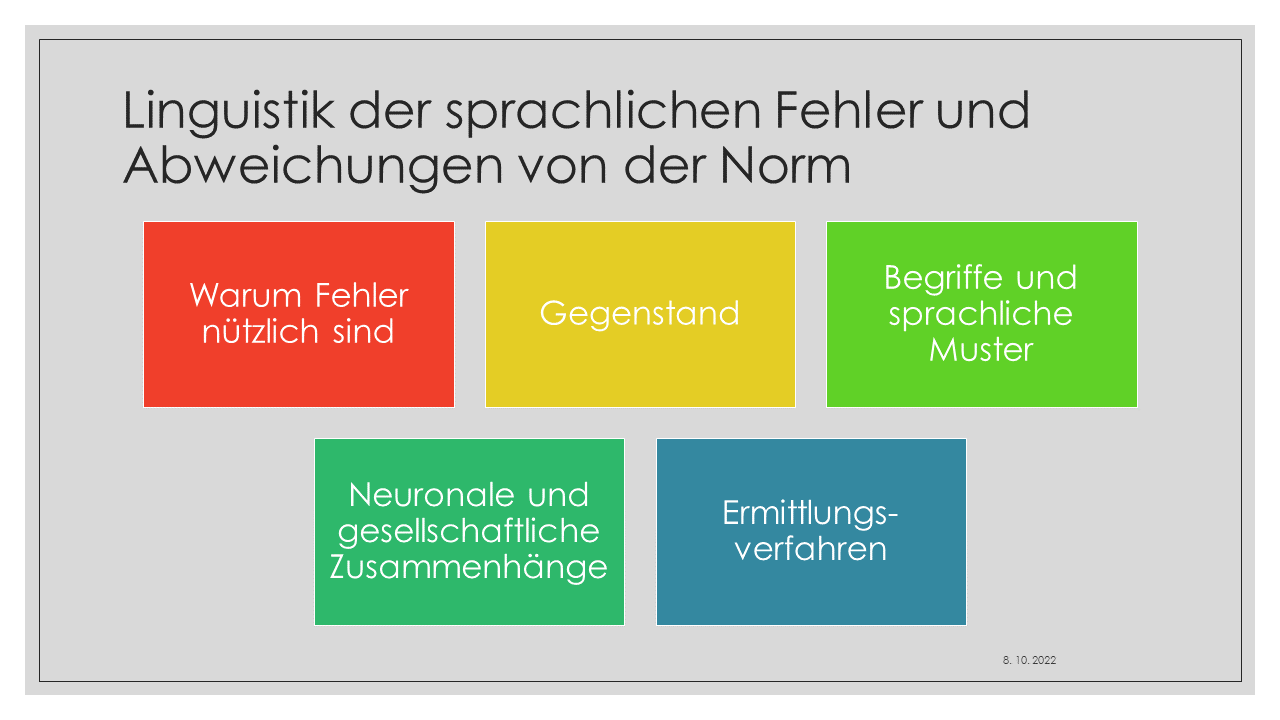
\includegraphics[width=1\textwidth,height=\textheight]{./pictures/Diapozitiv5.PNG}

In diesem Einführungskurs machen wir Sie mit grundlegenden Methoden zur
Erfassung von linguistischen Merkmalen in deutschen (und in einigen
Abschnitten auch mit slowenischen) Texten bekannt.\footnote{Dieses Buch
  wurde mit \texttt{Quarto} \url{https://quarto.org/docs/books/}
  zusammengestellt.}

Hinweise\footnote{Clipart von \url{https://www.clipartmax.com/}}:

Das ist eine Definition (rmdnote).

Das ist ein Tip oder eine Info (rmdtip).

Das ist ein Arbeitsvorschlag (rmdrobot).

Das ist der RStudio Logotyp (rmdrstudio).

Das ist eine Warnung (rmdwarning).

Das ist eine Fehlermeldung (rmderror).

\part{Teil 2:Fehler in der Zweit- / Fremdsprache}

\hypertarget{sec-l2_fehler}{%
\chapter{Fehler in Zweit- und Fremdsprache}\label{sec-l2_fehler}}

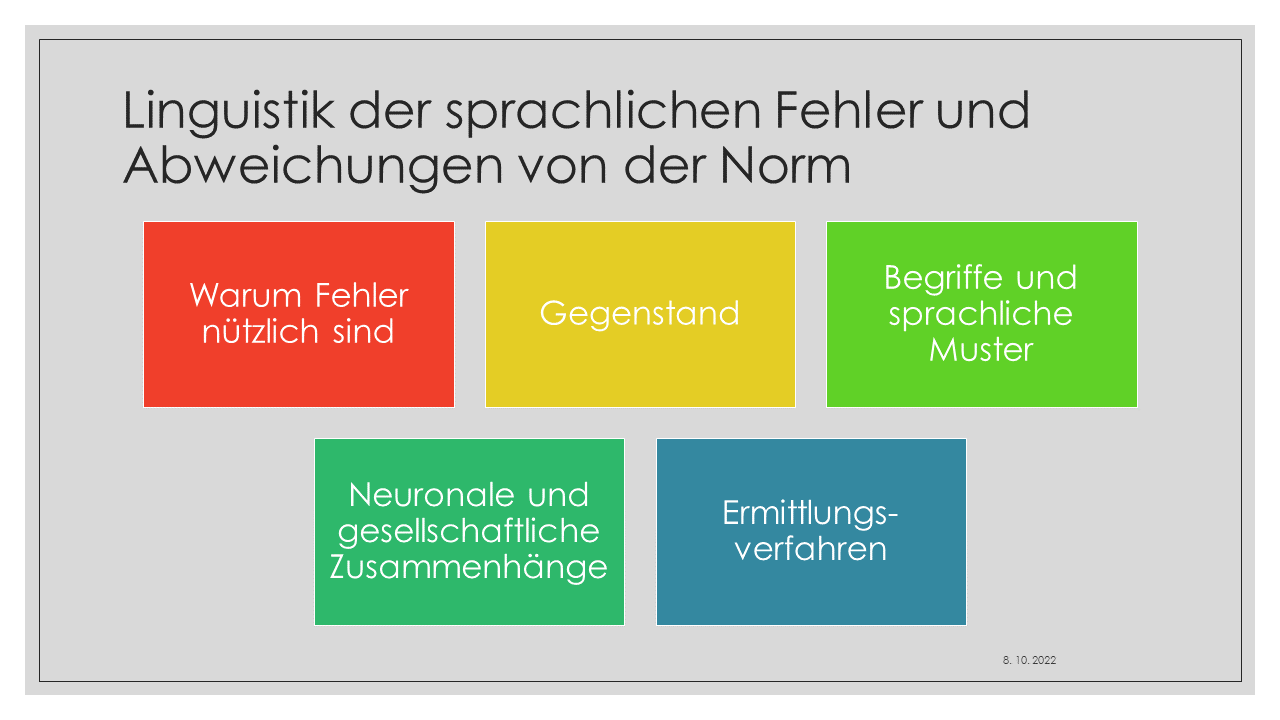
\includegraphics[width=1\textwidth,height=\textheight]{./pictures/Diapozitiv5.PNG}

In diesem Einführungskurs machen wir Sie mit grundlegenden Methoden zur
Erfassung von linguistischen Merkmalen in deutschen (und in einigen
Abschnitten auch mit slowenischen) Texten bekannt.\footnote{Dieses Buch
  wurde mit \texttt{Quarto} \url{https://quarto.org/docs/books/}
  zusammengestellt.}

Hinweise\footnote{Clipart von \url{https://www.clipartmax.com/}}:

Das ist eine Definition (rmdnote).

Das ist ein Tip oder eine Info (rmdtip).

Das ist ein Arbeitsvorschlag (rmdrobot).

Das ist der RStudio Logotyp (rmdrstudio).

Das ist eine Warnung (rmdwarning).

Das ist eine Fehlermeldung (rmderror).

\bookmarksetup{startatroot}

\hypertarget{summary}{%
\chapter{Summary}\label{summary}}

In summary, this book has no content whatsoever.

\begin{verbatim}
[1] 2
\end{verbatim}

\bookmarksetup{startatroot}

\hypertarget{references}{%
\chapter*{References}\label{references}}
\addcontentsline{toc}{chapter}{References}

\hypertarget{refs}{}
\begin{CSLReferences}{0}{0}
\end{CSLReferences}


\backmatter

\printindex

\end{document}
